\documentclass [a4paper] {article}
\usepackage[utf8]{inputenc}
\title{Ciencia de datos, práctica 4}
\author{Juan Casado Ballesteros, Samuel García Gonzalez, Iván Anaya Martín}
\usepackage{Sweave}
\begin{document}
\maketitle

\begin{abstract}
A lo largo de esta práctica analizaremos y compararemos distintos métodos de clasificación no supervisada o clusterización.

Utilizaremos el algoritmo de k-mean para realizar el ejercicio propuesto y la primera parte del ejercicio libre.
Nos centraremos principalmente en las técnicas de selección del número de clusters óptimo para lo cual exploraremos tres de ellas.
Adicionalmente hemos relizado una implementación propia de k-means que validaremos comparándola con los resultados de la implementación de R.
La ventaja de nuestra implementación frente a la de R es que nos permite visualizar paso a paso el estado de cada iteración del algoritmo.
Esto nos permite ver cómo se desplazan los centroides así como ver en cada momento la clasificación actual de los elementos de la muestra.

En la segunda parte del ejercicio libre utilizaremos los algoritmos de clasificación jerárquica aglomerativo y divisivo.
En el algoritmo aglomerativo partimos de que cada elemento de la muestra es una clases.
En cada iteración elegiremos las dos clases más próximas y la uniremos en una nueva clase creando así una estructura de árbol.
En el algoritmo divisivo todos los elementos serán consderados una única clase al inicio de la ejecución.
En cada iteración separaremos la clase en dos pudiendo contener cada una de ellas uno o más elementos creando así una estructura de árbol.
Las principales variaciones en estos métodos residen en la métrica utilizada para calcular la distancia entre clases a partir de la cual decidimos cuando separarlas o unirlas.
Exploraremos distintas métricas, visualizaremos los árboles generados y compararemos las clasificaciones jerárquicas entre si y con los resultados de k-means.

Debido a que deseamos comparar los resultados de k-means con la clasificación jerarquica utilizaremos para explorar ambos algoritmos el mismo dataset.
Este es un dataset ya incluido en R que tiene la cantidad de veces que 4 crímenes distintos se han cometido en cada estado de EEUU.
\end{abstract}

\newpage
\tableofcontents


\newpage
\section{K-means sobre la muestra proporcionada}

Aplicaremos el algoritmo k-means sobre la muestra que se nos proporciona.
Este algoritmo clasificará de forma no supervisada la muestra en tantas clases como indiquemos.
En primer lugar deberemos cargar esta desde un archivo .txt.
\begin{Schunk}
\begin{Sinput}
> datos1 <- read.table("datos1.txt")
> datos1
\end{Sinput}
\begin{Soutput}
  Teoria Laboratorio
1      4           4
2      3           5
3      1           2
4      5           5
5      0           1
6      2           2
7      4           5
8      2           1
\end{Soutput}
\end{Schunk}

Para esta muestra tal y como podemos ver y tal y como vimos en clase el número adecuado de centroides es 2.
Ubicaremos dos puntos a partir de los cuales se ejecutará el algoritmo.
\begin{Schunk}
\begin{Sinput}
> centroides <- matrix(c(0,1,2,2),2,2)
> centroides <- t(centroides)
> centroides
\end{Sinput}
\begin{Soutput}
     [,1] [,2]
[1,]    0    1
[2,]    2    2
\end{Soutput}
\end{Schunk}

Realizamos la ejecución del algoritmo con la implementación que R nos proporciona.
\begin{Schunk}
\begin{Sinput}
> classkms<-kmeans(datos1,centroides,4)
\end{Sinput}
\end{Schunk}

\subsection{Evaluación de la solución obtenida}
Podemos ver a que clase pertenecen cada uno de los elementos de la muestra.
Nuestra muestra tiene un total de ocho elementos que se han clasificado en dos clases (clase 1 y clase 2).
\begin{Schunk}
\begin{Sinput}
> classkms$cluster
\end{Sinput}
\begin{Soutput}
1 2 3 4 5 6 7 8 
2 2 1 2 1 1 2 1 
\end{Soutput}
\end{Schunk}
Centroides de cada una de las dos clases.
Son los puntos que minimizan las distancias a los elementos de la muestra, desde ellos a los elementos de su clase.
\begin{Schunk}
\begin{Sinput}
> classkms$centers
\end{Sinput}
\begin{Soutput}
  Teoria Laboratorio
1   1.25        1.50
2   4.00        4.75
\end{Soutput}
\end{Schunk}
Cantidad de elementos que pertenecen a cada una de las clases obtenidas.
\begin{Schunk}
\begin{Sinput}
> classkms$size
\end{Sinput}
\begin{Soutput}
[1] 4 4
\end{Soutput}
\end{Schunk}
Iteraciones necesarias para realizar la clasificación. Este valor no se refiere a las iteraciones del algoritmo,
con una sola iteración no se hubiera podido llegar a la solución.
\begin{Schunk}
\begin{Sinput}
> classkms$iter
\end{Sinput}
\begin{Soutput}
[1] 1
\end{Soutput}
\end{Schunk}
Indica si la clasificación obtenida es válida o no.
K-means con unos centroides iniciales mal-intencionadamente elegidos puede no llegar a una solución válida
\begin{Schunk}
\begin{Sinput}
> classkms$ifault
\end{Sinput}
\begin{Soutput}
[1] 0
\end{Soutput}
\end{Schunk}
Distancia cuadrática media entre los centroides, deseamos que este valor sea alto ya que querríamos que nuestros clusters fueran heterogéneos y bien diferenciados.
\begin{Schunk}
\begin{Sinput}
> classkms$betweenss
\end{Sinput}
\begin{Soutput}
[1] 36.25
\end{Soutput}
\end{Schunk}
Distancia cuadrática media dentro de cada cluster, deseamos obtener valores bajos, es decir, dentro de cada cluster los elementos deben estar próximos, deben ser homogéneos.
\begin{Schunk}
\begin{Sinput}
> classkms$withinss
\end{Sinput}
\begin{Soutput}
[1] 3.75 2.75
\end{Soutput}
\end{Schunk}
Suma de todas las distancias cuadráticas medias dentro de los clusters.
\begin{Schunk}
\begin{Sinput}
> classkms$tot.withinss
\end{Sinput}
\begin{Soutput}
[1] 6.5
\end{Soutput}
\end{Schunk}
Suma de todas las distancias cuadráticas medias dentro de los clusters y la distancia cuadrática media entre clusters.
\begin{Schunk}
\begin{Sinput}
> classkms$totss
\end{Sinput}
\begin{Soutput}
[1] 42.75
\end{Soutput}
\end{Schunk}
Estos últimos cuatro valores ayudan a decidir si el algoritmo ha realizado una clasificación correcta o no.

\subsection{Visualización del resultado}
Dividiremos la muestra en las clases que la ejecución nos ha proporcionado.
Dibujaremos dichas clases junto a sus representantes en una gráfica bidimensional.
Primero deberemos separar los elemntos de la muestra según la clasificación btenida.
\begin{Schunk}
\begin{Sinput}
> clusters <- cbind(classkms$cluster,datos1)
> cluster1 <- subset(clusters,clusters[,1]==1)
> cluster2 <- subset(clusters,clusters[,1]==2)
> cluster1 <- cluster1[,-1]
> cluster2 <- cluster2[,-1]
> clusters <- list(cluster1, cluster2)
\end{Sinput}
\end{Schunk}

Como podemos ver la clasificación se ha realizado correctamente.
\begin{center}
\includegraphics{entrega-representacion_del_resultado}
\end{center}

\subsection{Pasos de la clasificación}
Aunque establezcamos una iteración como número máximo de iteraciones al lanzar el algoritmo este siempre llega a la solución final sin proporcionar los pasos intermedios.
Es por ello que decidimos implementar nuestra propia versión de k-means con la intención de poder mostrar estos pasos intermedios.
A cada iteración del algoritmo extraemos y mostramos el estado de la ejecución en una gráfica distinta.
Podemos ver la evolución de los centroides desde sus posiciones iniciales hasta las finales.
Comprobamos que el resultado de la ejecución con nuestra implementación coincide con el de la implementación de R.
\begin{center}
\begin{Schunk}
\begin{Sinput}
> current_centroides <- centroides
> par(mfrow=c(2,2))
> for (i in 1:4){
+   cluster <- kmeans_cluster (datos1, current_centroides)
+   split <- kmeans_split(datos1, cluster)
+   new_centroides <- kmeans_new_centroids(split)
+   plot_kmeans(split, current_centroides, main=toString(i),
+               xlab="Teroría", ylab="Laboratorio")
+   if (same_centroids(new_centroides, current_centroides)){
+     break
+   }else{
+     current_centroides <- new_centroides
+   }
+ }
> current_centroides
\end{Sinput}
\begin{Soutput}
     [,1] [,2]
[1,] 1.25 1.50
[2,] 4.00 4.75
\end{Soutput}
\end{Schunk}
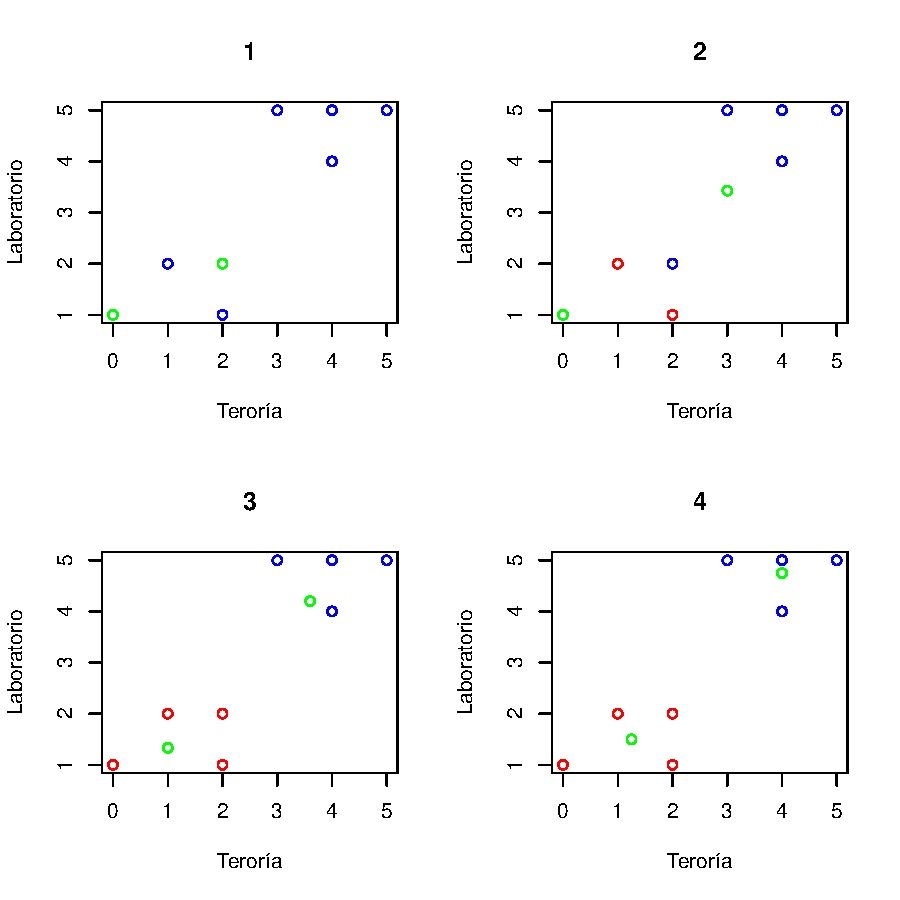
\includegraphics{entrega-custom_kmeans}
\end{center}

\newpage
\section{K-means}
En este apartado vamos a realizar un ejemplo práctico de clustering de la muestra "USArrests" incluida en R.
Utilizaremos distintas funciones de las librerías: "tidyverse", "cluster", "factoextra" y "gridExtra" para mostrar los datos y calcular el número óptimo de clusters.
El algoritmo encargado de realizar la clusterización será kmeans del que utilizaremos la implementación que R proporciona.

La muestra que se utilizará contiene la cantidad de veces que se han cometido 4 crímenes distintos en distintos estados de EEUU.

\subsection{Preparar los datos}
Deberemos eliminar los datos que estén incompletos ya que kmeans no podría manejarlos.
Adicionalmente escalaremos las variables con la intención de hacerlas comparables entre ellas.
Esto es necesario debido a que la escala de las variables de entrada adecta al algoritmo pues se utilizar distancias euclídeas para realizar la clusterización.
Escalar las variables consiste en hacer que la media de cada una de ellas sea 0 y desviación estándar de 1.
Es por ello que se acaban obteniendo valores negativos para las variables, tendría poco sentido que se hubiera cometido una cantidad negativa de crímenes en un estado.
\begin{Schunk}
\begin{Sinput}
> df <- read.csv("Seed_Data.csv")
> df <- na.omit(df)
> df <- scale(df)
\end{Sinput}
\end{Schunk}
Mostraramos a continuación un extracto de los datos.
\begin{Schunk}
\begin{Sinput}
> head(df)
\end{Sinput}
\begin{Soutput}
            A            P            C          LK        WK     A_Coef
1  0.14175904  0.214948819 6.045733e-05  0.30349301 0.1413640 -0.9838010
2  0.01116136  0.008204153 4.274938e-01 -0.16822270 0.1969616 -1.7839036
3 -0.19160873 -0.359341919 1.438945e+00 -0.76181710 0.2075516 -0.6658882
4 -0.34626388 -0.474200066 1.036904e+00 -0.68733567 0.3187467 -0.9585276
5  0.44419577  0.329806966 1.371233e+00  0.06650665 0.8032397 -1.5597684
6 -0.16067770 -0.267455401 1.019976e+00 -0.54740087 0.1413640 -0.8235144
         LKG    target
1 -0.3826631 -1.221825
2 -0.9198156 -1.221825
3 -1.1863572 -1.221825
4 -1.2270506 -1.221825
5 -0.4742231 -1.221825
6 -0.9198156 -1.221825
\end{Soutput}
\end{Schunk}

\newpage
\subsection{Conocer los datos}
Antes de poder realizar cualquier análisis de datos debemos de conocerlos.
En este caso utilizaremos una matriz de distancias para poder hacerlo.
Dicha matriz nos mostrará las distancias entre los elementos que manejamos.
En ella podemos observar que las distancias son heterogéneas entre los elementos, es decir, hay variedad de distancias.
Entre otras cosas la matriz puede ayudarnos a elegir una distancia euclídea para realizar con ella la clasificación seleccionando una que acentúe las desigualdades entre clases.
\begin{center}
\begin{Schunk}
\begin{Sinput}
> dist <- get_dist(df)
> fviz_dist(dist, gradient = list(low = "#00AFBB", mid = "white", high = "#FC4E07"))
\end{Sinput}
\end{Schunk}
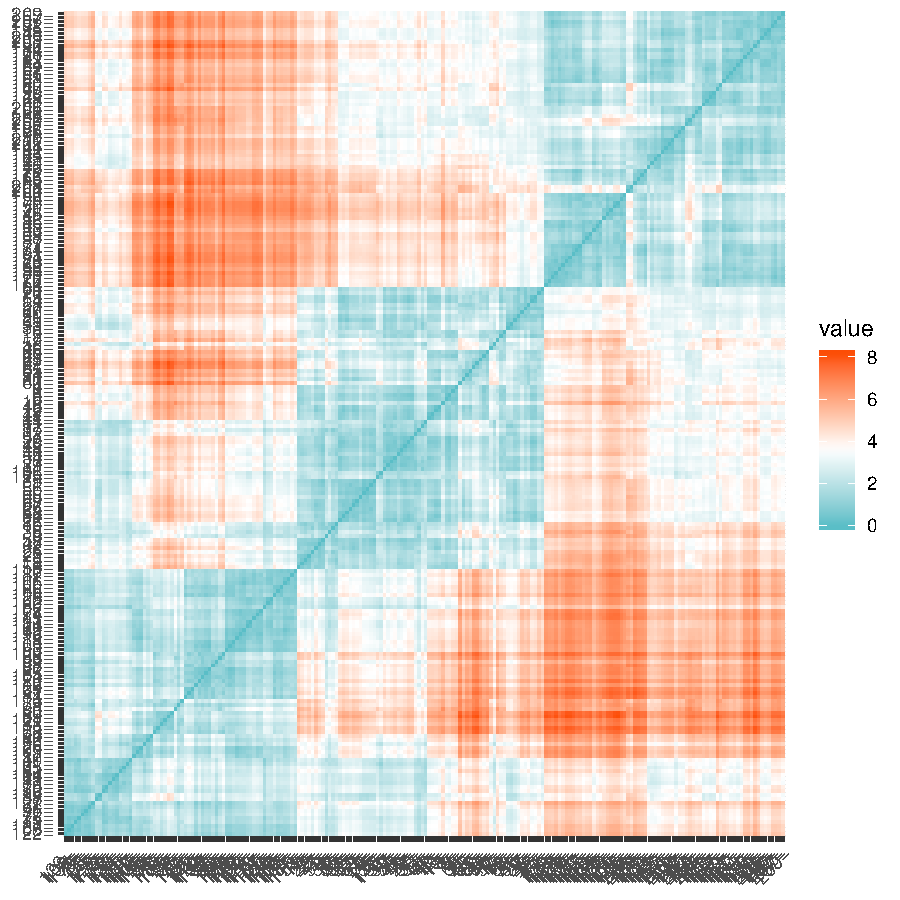
\includegraphics{entrega-kmeans_distances}
\end{center}

\newpage
\subsection{Ejecución del algoritmo}
Ejecutaremos el algoritmo kmeans implementado en R.
En este caso en vez de fijar nosotros los centroides iniciales indicaremos que queremos obtener 2 clases distintas siendo el propio algoritmo quien los establezca.
Adicionalmente indicaremos que queremos probar un total de 25 combinaciones de centroides iniciales.
Dependidendo de las posiciones iniciales obtendremos distintos resultados en la clasificación, ejecuatando el algoritmo varias veces nos aseguramos de quedarnos con una clusterización adecuada.
\begin{Schunk}
\begin{Sinput}
> k2 <- kmeans(df, centers = 2, nstart = 25)
\end{Sinput}
\end{Schunk}
Obtenemos dos centroides, uno para cada clase, además visualizamos la cantidad de elementos en cada una de las clases.
\begin{Schunk}
\begin{Sinput}
> k2$centers
\end{Sinput}
\begin{Soutput}
           A          P          C         LK         WK     A_Coef        LKG
1 -0.7291716 -0.7302497 -0.4033226 -0.7036119 -0.7025866  0.1381082 -0.6853159
2  1.0308978  1.0324220  0.5702148  0.9947616  0.9933121 -0.1952564  0.9688949
      target
1  0.1688702
2 -0.2387475
\end{Soutput}
\begin{Sinput}
> k2$size
\end{Sinput}
\begin{Soutput}
[1] 123  87
\end{Soutput}
\end{Schunk}
Adicionalmente mostramos las distancias cuadráticas medias entre los elementos de cada cluster y entre los clusters.
Utilizaremos estas medidas posteriormente para compararlas con la clasificación mediante otros números de clusters.
\begin{Schunk}
\begin{Sinput}
> k2$withinss
\end{Sinput}
\begin{Soutput}
[1] 578.4479 281.9642
\end{Soutput}
\begin{Sinput}
> k2$betweenss
\end{Sinput}
\begin{Soutput}
[1] 811.5879
\end{Soutput}
\end{Schunk}

Mostramos la clasificación obtenida.
\begin{center}
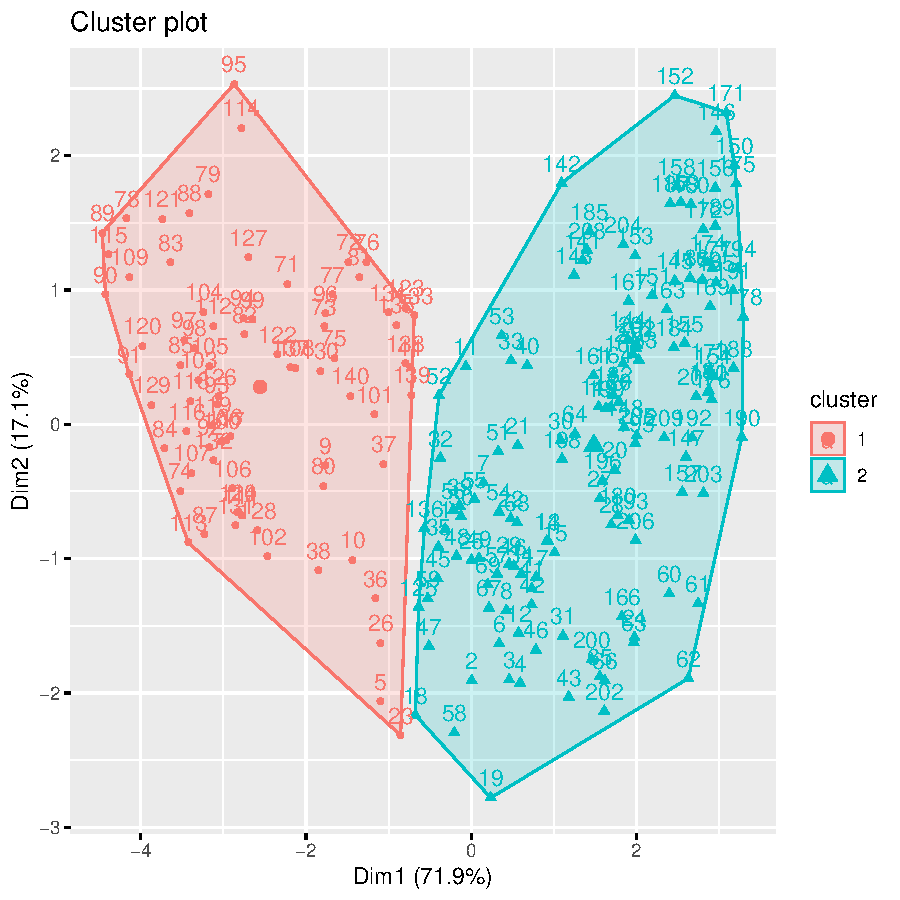
\includegraphics{entrega-kmeans_show_resultse}
\end{center}

\newpage
\subsection{Ejecución con implementación propia}
Realizaremos la misma ejecución utilizando ahora la implementación de kmeans hecha por nosotros.
En este caso debemos elegir nosotros los centrides iniciales que serán 2 centroides de 4 elementos cada uno.
Tras la ejecución podremos ver en las gráficas como los centroides logran clasificar los elementos en 5 iteraciones.
Adicionalmente podemos comprobar que los centrides obtenidos con nuestra implementación y con la de R son los mismos.
\begin{center}
\begin{Schunk}
\begin{Sinput}
> datos <- df
> current_centroides <- matrix(runif(16, -2, 2), 2,8)
> par(mfrow=c(2,3))
> for (i in 1:6){
+   cluster <- kmeans_cluster (datos, current_centroides)
+   split <- kmeans_split(datos, cluster)
+   new_centroides <- kmeans_new_centroids(split)
+   plot_kmeans(split, current_centroides, main=toString(i),
+               xlab="Teroría", ylab="Laboratorio")
+   if (same_centroids(new_centroides, current_centroides)){
+     break
+   }else{
+     current_centroides <- new_centroides
+   }
+ }
> current_centroides
\end{Sinput}
\begin{Soutput}
           [,1]       [,2]       [,3]       [,4]      [,5]       [,6]
[1,]  0.6452339  0.6391703  0.5202648  0.5885697  0.662255 -0.3346674
[2,] -0.9872857 -0.9780076 -0.7960679 -0.9005826 -1.013330  0.5120814
           [,7]       [,8]
[1,]  0.4498369 -0.5483783
[2,] -0.6883046  0.8390849
\end{Soutput}
\end{Schunk}
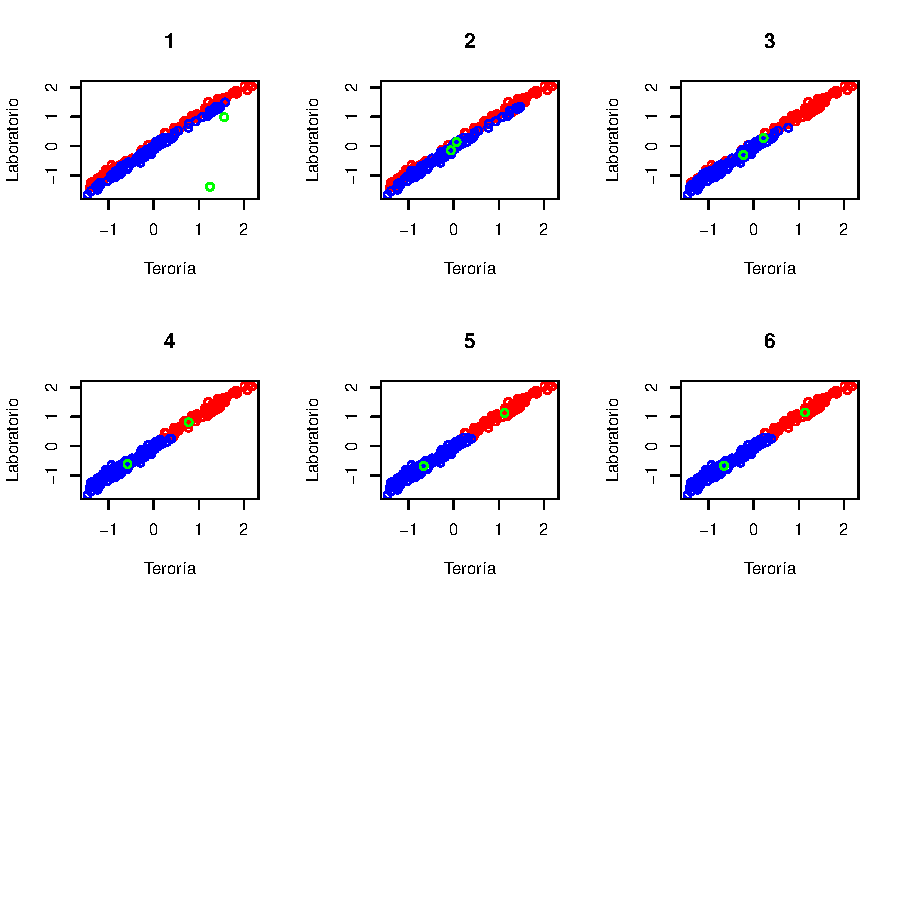
\includegraphics{entrega-kmeans_our_implementation}
\end{center}

Comprobamos adicionalmente que ambas clasificaciones, la de R y la nuestara coinciden como método de validación de nuestro algoritmo.
El resultado es positivo.
\begin{Schunk}
\begin{Sinput}
> clusters <- cbind(k2$cluster,datos)
> cluster1 <- subset(clusters,clusters[,1]==1)
> cluster2 <- subset(clusters,clusters[,1]==2)
> cluster1 <- cluster1[,-1]
> cluster2 <- cluster2[,-1]
> clusters <- list(cluster1, cluster2)
> len <- length(clusters)
> same1 = 0
> for (i in 1:len){
+   r_results = clusters[[i]]
+   our_results = split[[i]]
+   if (nrow(r_results) < nrow(our_results)){
+     temp <- r_results
+     r_results <- our_results
+     our_results <- temp
+   }
+   for (name in rownames(r_results)){
+     if (name %in% rownames(our_results)){
+       same1 <- same1+1
+     }
+   }
+ }
> same2 = 0
> for (i in 1:len){
+   r_results = clusters[[i]]
+   our_results = split[[((i)%%len)+1]]
+   if (nrow(r_results) < nrow(our_results)){
+     temp <- r_results
+     r_results <- our_results
+     our_results <- temp
+   }
+   for (name in rownames(r_results)){
+     if (name %in% rownames(our_results)){
+       same2 <- same2+1
+     }
+   }
+ }
> max(same1,same2)/nrow(datos)
\end{Sinput}
\begin{Soutput}
[1] 0.8095238
\end{Soutput}
\end{Schunk}

\newpage
\subsection{Elección del número de clusters}
Hasta ahora hemos elegido siempre 2 como el número de clusters.
No obstante esta decisión no debiera ser trivial.
Expondremos a continuación una serie de métodos que pueden guiarnos a la hora de tomar esta decisión.

\subsubsection{Elbow Method}
Este método se basa en calcular la suma de las distancias cuadráticas medias entre los elementos de los clusters y dibujarlas en una gráfica.
Este valor es el proporcionado en "tot.withinss" al ejecutar kmeans tal y como ya explicamos en el primer apartado.
En la gráfica el número de cluster óptimos será aquel en el que se produzca un codo en la gráfica.
La suma de las distancias se irá reduciendo hasta llegar a 0 cuando haya tantas clases como elementos.
El punto de nuestro interés está en el momento en el que la gráfica comienza a descender a un ritmo menor.
\begin{center}
\begin{Schunk}
\begin{Sinput}
> wss <- function(k) {
+   kmeans(df, k, nstart = 10 )$tot.withinss
+ }
> k.values <- 1:15
> wss_values <- map_dbl(k.values, wss)
> plot(k.values, wss_values,
+        type="b", pch = 19, frame = FALSE, 
+        xlab="Number of clusters K",
+        ylab="Total within-clusters sum of squares")
\end{Sinput}
\end{Schunk}
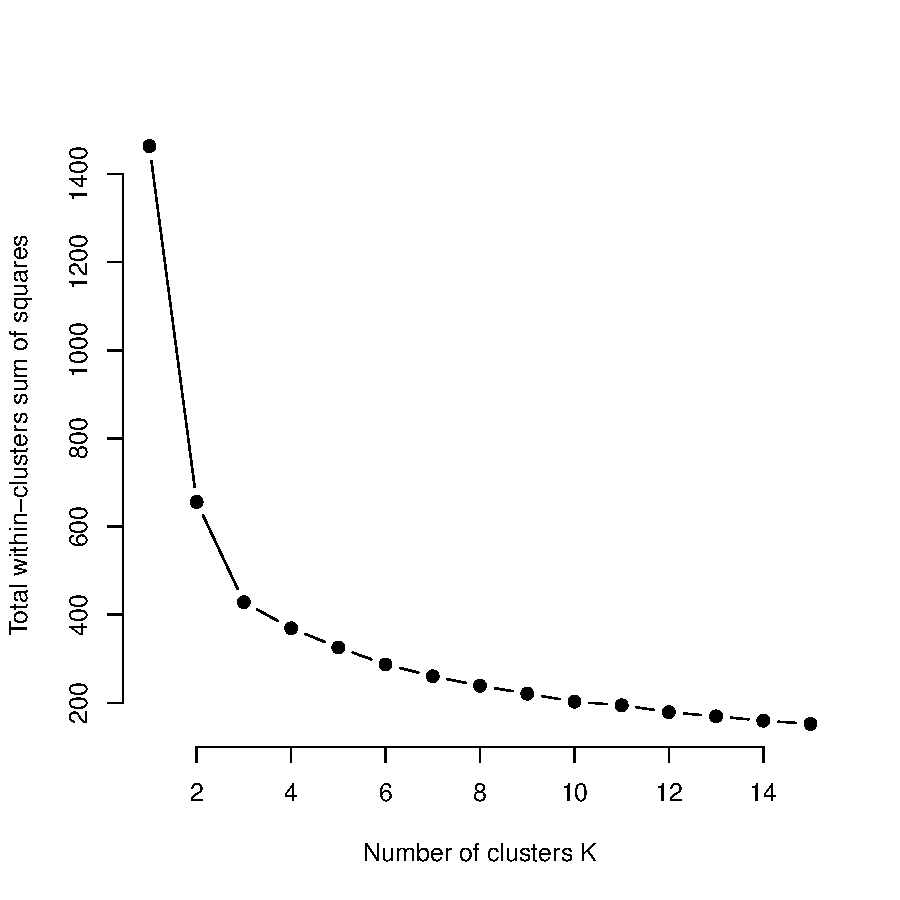
\includegraphics{entrega-optimal_number_of_clusters_1}
\end{center}
La siguiente función ya implementa este método de modo que no es necesario realizarlo manualmente.
\begin{center}
\begin{Schunk}
\begin{Sinput}
> fviz_nbclust(df, kmeans, method = "wss")
\end{Sinput}
\end{Schunk}
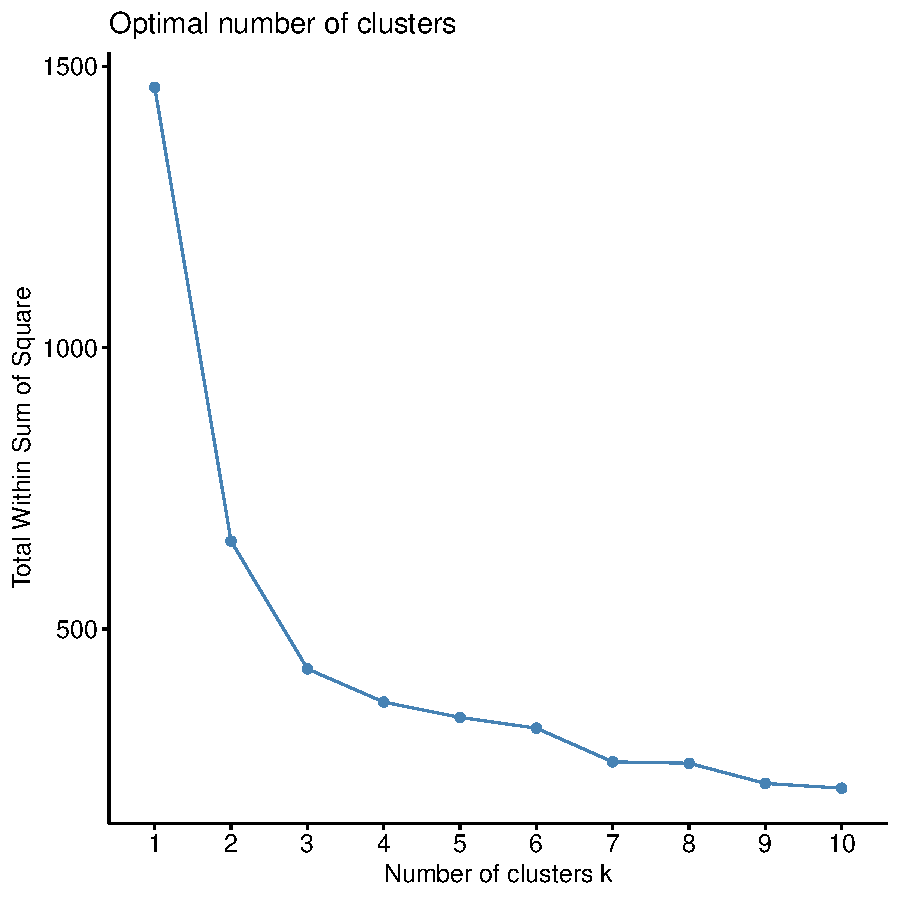
\includegraphics{entrega-optimal_number_of_clusters_2}
\end{center}

Podemos ver que el número de clusters óptimo estaría entre los valores de 2 y 4 clases.

\subsubsection{Average Silhouette Method}
Este método trata de calcular la paertenencia de cada elemento al cluster en el que ha sido clasificado.
Lo calcularemos manualmente para los valores de 2 a 15 clases.
Buscamos en esta gráfica aquellos números de clusters que maximizan la pertencencia de sus elementos.
\begin{center}
\begin{Schunk}
\begin{Sinput}
> avg_sil <- function(k) {
+   km.res <- kmeans(df, centers = k, nstart = 25)
+   ss <- silhouette(km.res$cluster, dist(df))
+   mean(ss[, 3])
+ }
> k.values <- 2:15
> avg_sil_values <- map_dbl(k.values, avg_sil)
> plot(k.values, avg_sil_values,
+        type = "b", pch = 19, frame = FALSE, 
+        xlab = "Number of clusters K",
+        ylab = "Average Silhouettes")
\end{Sinput}
\end{Schunk}
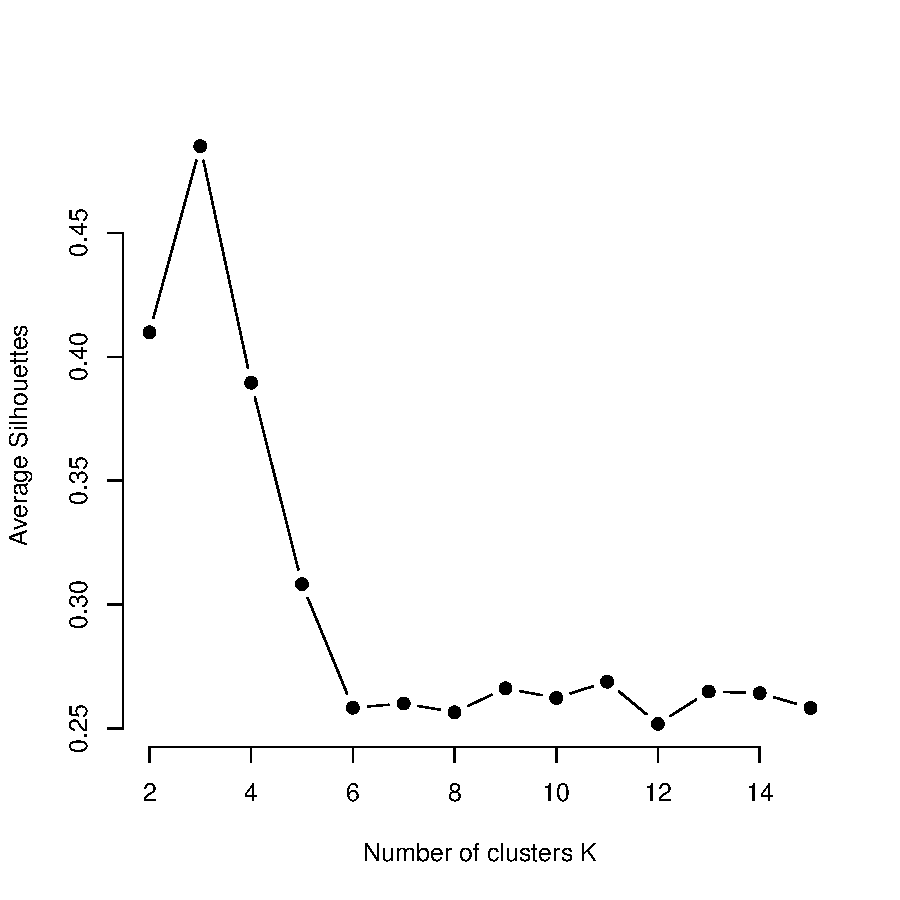
\includegraphics{entrega-optimal_number_of_clusters_3}
\end{center}
El mismo método está ya implementado en una única función.
\begin{center}
\begin{Schunk}
\begin{Sinput}
> fviz_nbclust(df, kmeans, method = "silhouette")
\end{Sinput}
\end{Schunk}
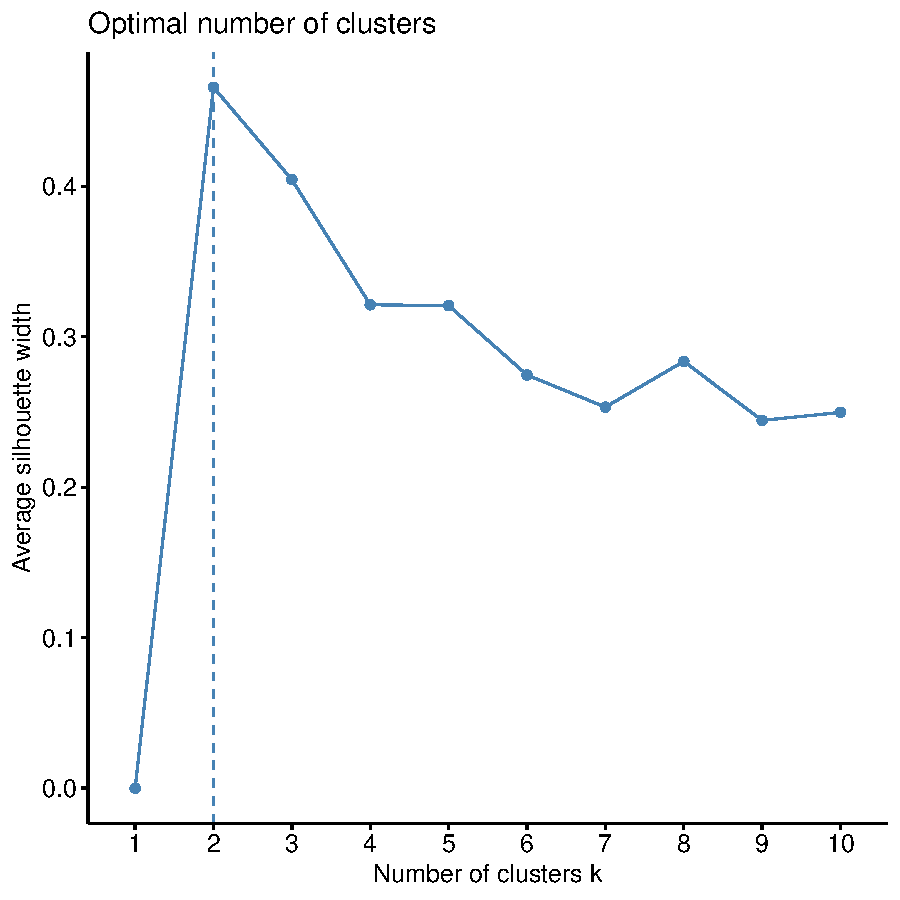
\includegraphics{entrega-optimal_number_of_clusters_4}
\end{center}

Podemos ver que 2 clases tiene la mayor pertenencia de los elementos clasificados a los clusters seguido de 4 clases.
Estos valores coinciden con los obtenidos con el método anterior.

\subsubsection{Gap Statistic Method}
Este es un método más complejo que los anteriores. La explicación del mismo puede verse en: http://web.stanford.edu/~hastie/Papers/gap.pdf.
Como resultados se obtiene una gráfica cuyo valor más alto será el mejor número de clusters.
Junto a cada valor se nos indica la calidad de la estimación.
Buscamos la combinación de un valor más alto en la gráfica con unos bigotes de menor tamaño.
\begin{center}
\begin{Schunk}
\begin{Sinput}
> gap_stat <- clusGap(df, FUN = kmeans, nstart = 25, K.max = 10, B = 50, verbose=FALSE)
> fviz_gap_stat(gap_stat)
\end{Sinput}
\end{Schunk}
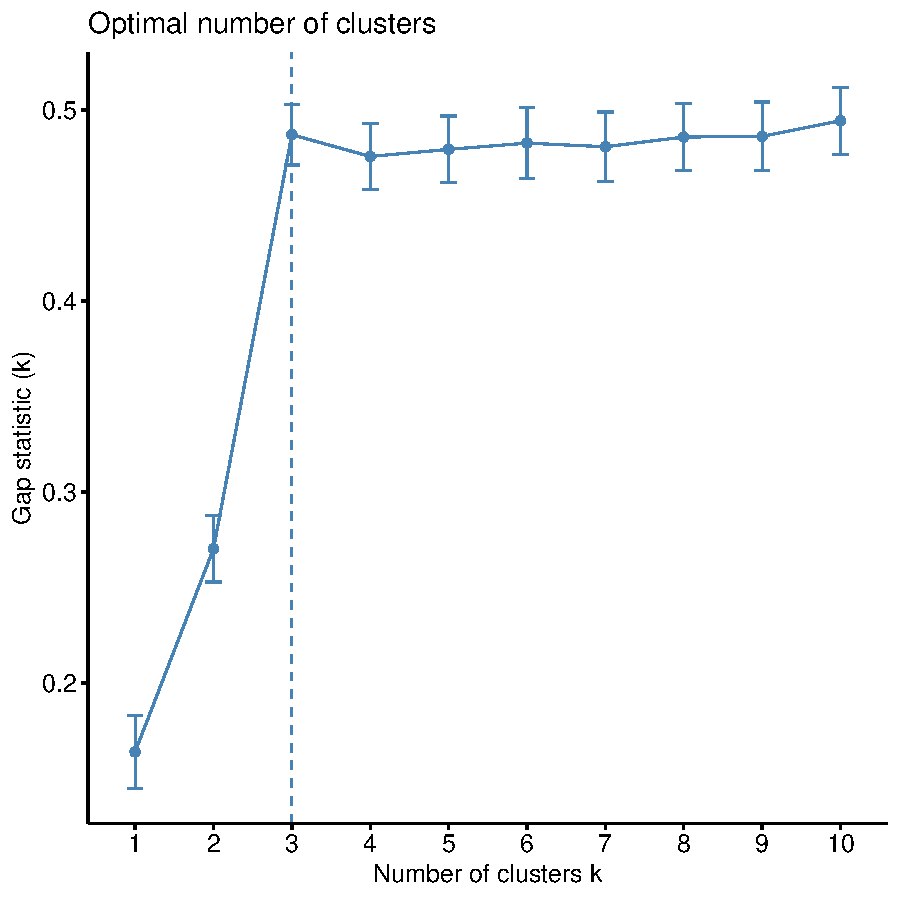
\includegraphics{entrega-optimal_number_of_clusters_5}
\end{center}

Podemos ver que en este caso 3 sería el mejor número de cluster en los que realizar nuestra clasificación.

Mostramos a continuación las distintas clasificciones que se obtienen cuando tenemos de 3 a 5 clases.
\begin{center}
\begin{Schunk}
\begin{Sinput}
> k3 <- kmeans(df, centers = 3, nstart = 25)
> k4 <- kmeans(df, centers = 4, nstart = 25)
> k5 <- kmeans(df, centers = 5, nstart = 25)
> p1 <- fviz_cluster(k2, geom = "point", data = df) + ggtitle("k = 2")
> p2 <- fviz_cluster(k3, geom = "point",  data = df) + ggtitle("k = 3")
> p3 <- fviz_cluster(k4, geom = "point",  data = df) + ggtitle("k = 4")
> p4 <- fviz_cluster(k5, geom = "point",  data = df) + ggtitle("k = 5")
> grid.arrange(p1, p2, p3, p4, nrow = 2)
\end{Sinput}
\end{Schunk}
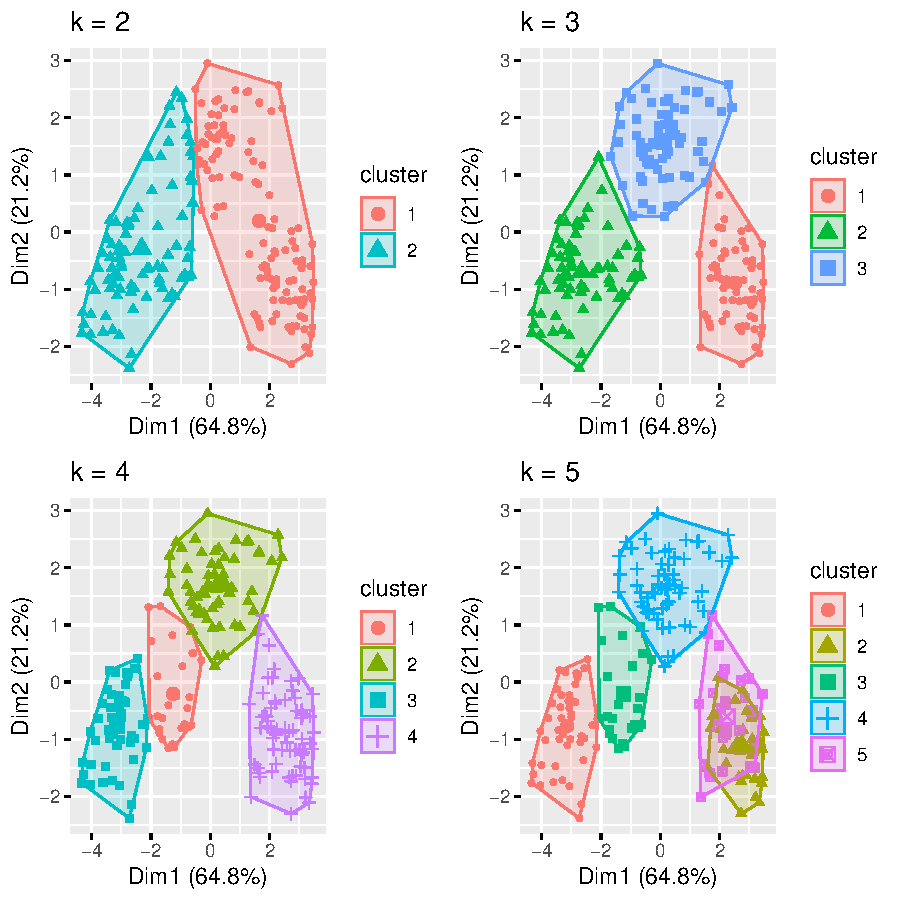
\includegraphics{entrega-kmeans_different_number_of_clusters}
\end{center}

Finalmente mostramos la suma de las distancias entre los elementos de los clusters y entre los clusters.
Vemos como al aumentar el número de clusters la calidad de la clasificación dentro de los clusters aumenta mientra que la calidad de la clasificación entre cluster disminuye.
Es por tanto que la elección del número de cluster es una optimización de estas dos variables teniendo en cuenta que puede que nos interese favorecer a una frente a la otra.
\begin{Schunk}
\begin{Sinput}
> c(k2$betweens, k3$betweens, k4$betweens, k5$betweens)
\end{Sinput}
\begin{Soutput}
[1]  811.5879 1217.4627 1271.8794 1318.4474
\end{Soutput}
\begin{Sinput}
> c(k2$tot.withinss, k3$tot.withinss, k4$tot.withinss, k5$tot.withinss)
\end{Sinput}
\begin{Soutput}
[1] 860.4121 454.5373 400.1206 353.5526
\end{Soutput}
\end{Schunk}

\newpage
\section{Clusterización jerárquica}
Utilizaremos y compararemos el método de clusterización jerárquica dependiendo de la medida de distancia que utilicemos para ejecuatarlo.
Utilizaremos funciones de las siguiente librerías: "cluster", "purrr", "dendextend" y "factoextra".

\begin{Schunk}
\begin{Sinput}
> data <- read.csv("Seed_Data.csv")
> data <- na.omit(data)
> data <- scale(data)
\end{Sinput}
\end{Schunk}

\begin{Schunk}
\begin{Sinput}
> d <- dist(data, method = "euclidean")
> hc1 <- hclust(d, method = "complete")
> plot(hc1, cex = 0.6, hang = -1)
\end{Sinput}
\end{Schunk}
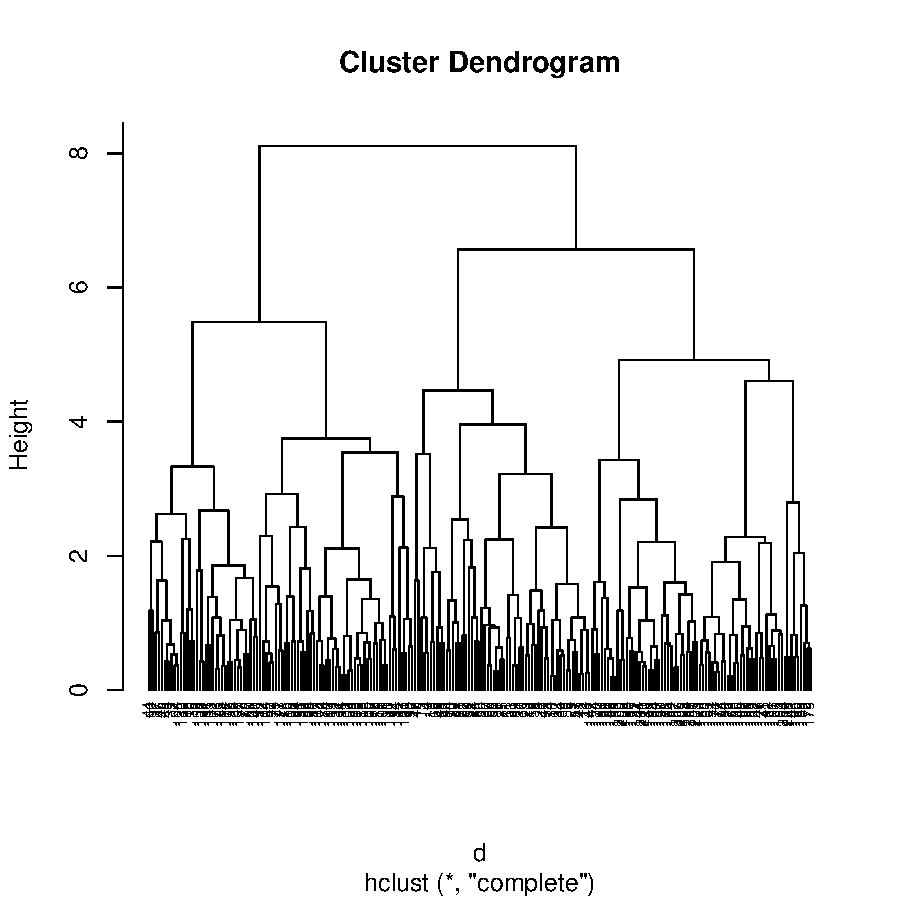
\includegraphics{entrega-jerarquico_1}

\begin{Schunk}
\begin{Sinput}
> hc2 <- agnes(data, method = "complete")
> hc2$ac
\end{Sinput}
\begin{Soutput}
[1] 0.9228468
\end{Soutput}
\begin{Sinput}
> m <- c( "average", "single", "complete", "ward")
> names(m) <- c( "average", "single", "complete", "ward")
> ac <- function(x) {
+   agnes(data, method = x)$ac
+ }
> map_dbl(m, ac)
\end{Sinput}
\begin{Soutput}
  average    single  complete      ward 
0.8705518 0.7471995 0.9228468 0.9843637 
\end{Soutput}
\begin{Sinput}
> hc3 <- agnes(data, method = "ward")
> pltree(hc3, cex = 0.6, hang = -1, main = "Dendrogram of agnes")
\end{Sinput}
\end{Schunk}
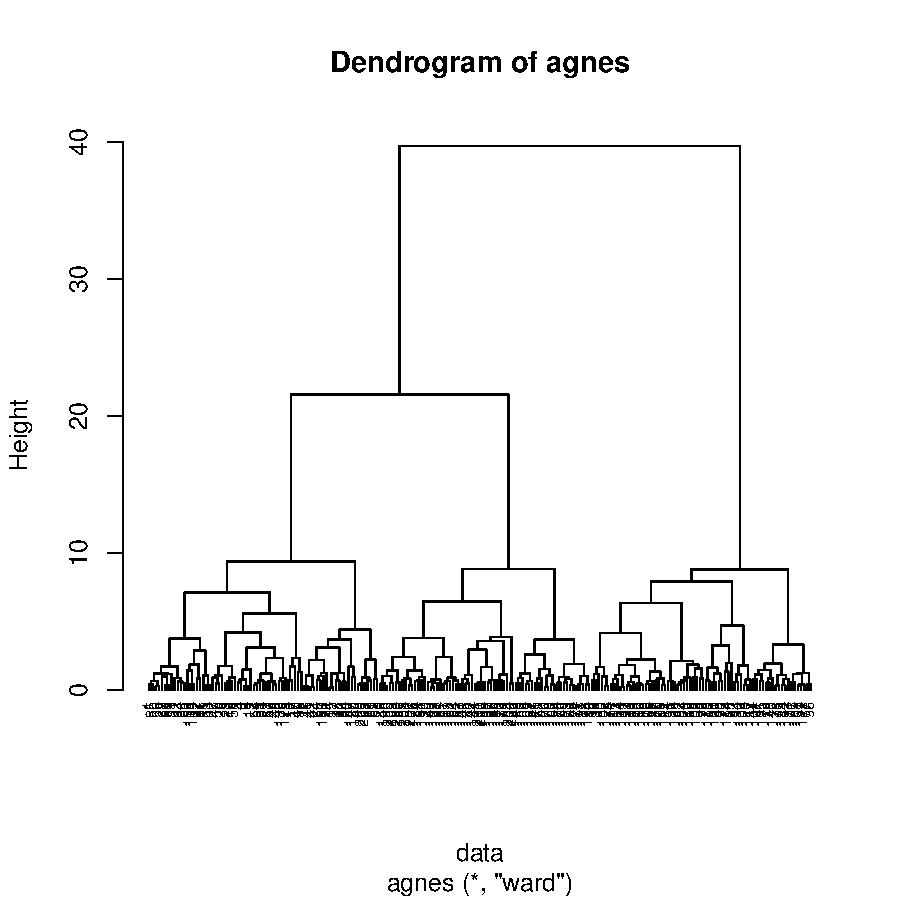
\includegraphics{entrega-jerarquico_2}

\begin{Schunk}
\begin{Sinput}
> hc4 <- diana(data)
> hc4$dc
\end{Sinput}
\begin{Soutput}
[1] 0.912948
\end{Soutput}
\begin{Sinput}
> pltree(hc4, cex = 0.6, hang = -1, main = "Dendrogram of diana")
\end{Sinput}
\end{Schunk}
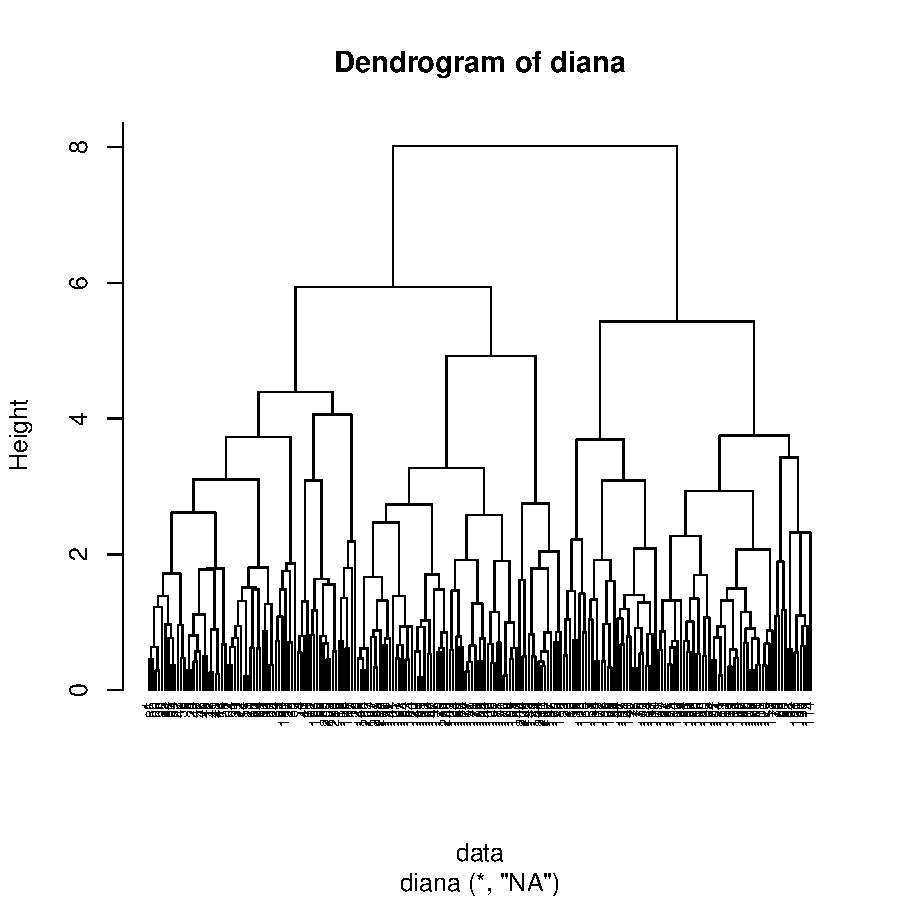
\includegraphics{entrega-jerarquico_3}

\begin{Schunk}
\begin{Sinput}
> clust <- cutree(hc4, k = 5)
> fviz_cluster(list(data = data, cluster = clust))
\end{Sinput}
\end{Schunk}
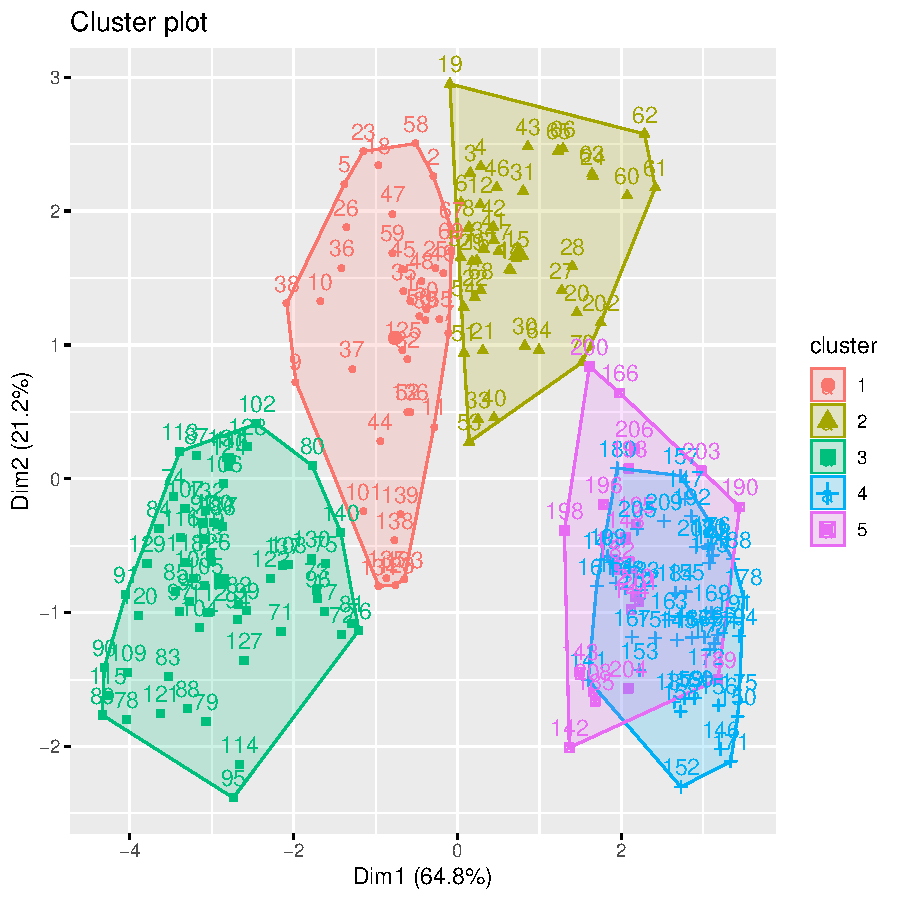
\includegraphics{entrega-jerarquico_4}

\begin{Schunk}
\begin{Sinput}
> pltree(hc4, hang=-1, cex = 0.6)
> rect.hclust(hc4, k = 9, border = 2:10)
\end{Sinput}
\end{Schunk}
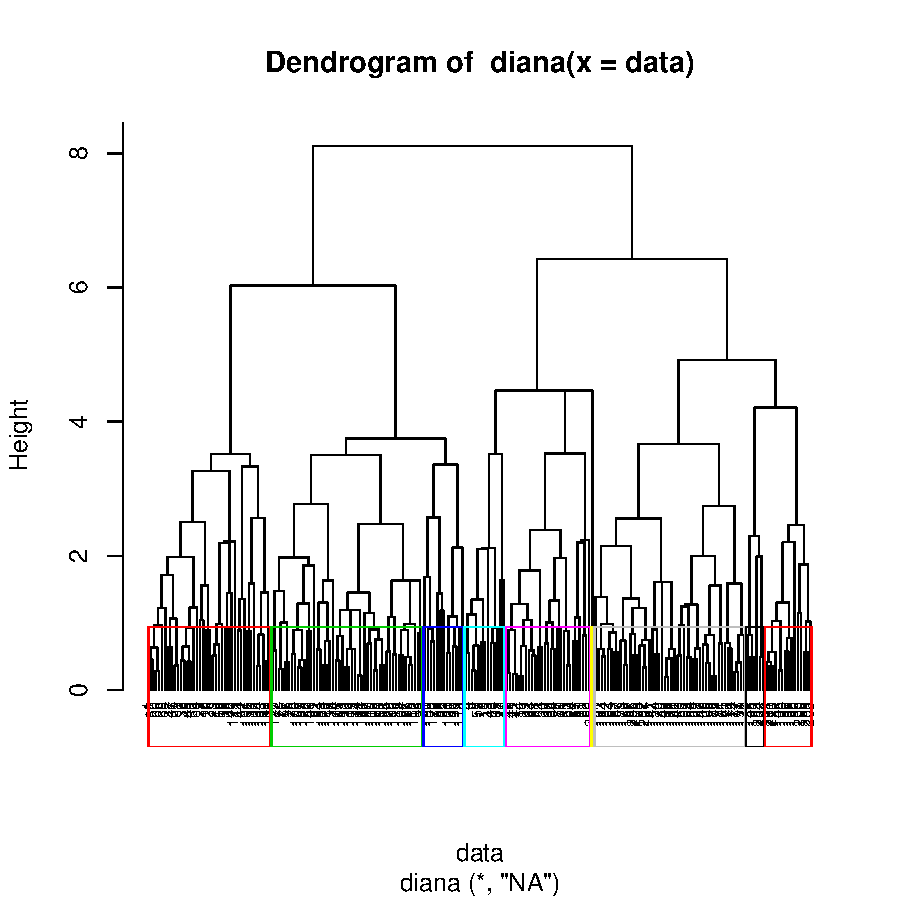
\includegraphics{entrega-jerarquico_5}
\begin{Schunk}
\begin{Sinput}
> hc_single <- agnes(data, method = "single")
> hc_complete <- agnes(data, method = "complete")
> hc_single <- as.dendrogram(hc_single)
> hc_complete <- as.dendrogram(hc_complete)
> tanglegram(hc_single,hc_complete)
\end{Sinput}
\end{Schunk}
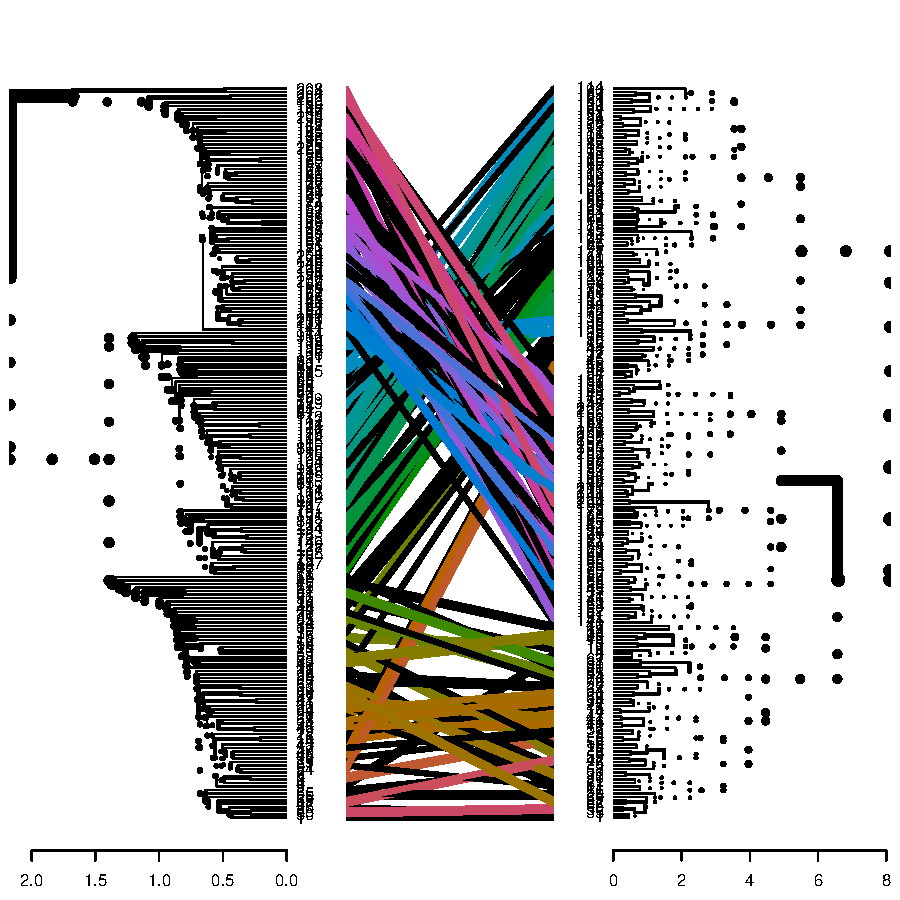
\includegraphics{entrega-jerarquico_6}

\newpage
\section{Funciones implementadas}
Las funcines creadas son las que implementan k-means así como una función adicional para crear las gráficas con los resultados.
\begin{Schunk}
\begin{Sinput}
> distance
\end{Sinput}
\begin{Soutput}
function (point1, point2) {
  acc <- 0
  len <- length(point1)
  for (i in 1:len){
    acc <- acc + (point1[i]-point2[i])^2
  }
  acc^(1/2)
}
<bytecode: 0x7ff9c6ec64a8>
\end{Soutput}
\begin{Sinput}
> kmeans_cluster
\end{Sinput}
\begin{Soutput}
function (data, centroids) {
  d_default <- distance(c(max(data), max(data)), c(min(data), min(data)))
  classification <- c()
  for (j in 1:nrow(data)){
      point <- data[j,]
      best_c <- 0
      best_d <- d_default
      for (i in 1:nrow(centroids)){
        centroid <- centroids[i,]
        d <- distance (point, centroid)
        if (d < best_d){
          best_d <- d
          best_c <- i
        }
    }
    classification <- c(classification, best_c)
  }
  classification <- as.data.frame(classification)
  rownames(classification) <- rownames(data)
  classification
}
<bytecode: 0x7ff9c7b7eee8>
\end{Soutput}
\begin{Sinput}
> kmeans_split
\end{Sinput}
\begin{Soutput}
function (data, cluster) {
  clusters=cbind(cluster,data)
  cluster1=subset(clusters,clusters[,1]==1)
  cluster2=subset(clusters,clusters[,1]==2)
  cluster1=cluster1[,-1]
  cluster2=cluster2[,-1]
  list(cluster1, cluster2)
}
<bytecode: 0x7ff9c763dff0>
\end{Soutput}
\begin{Sinput}
> kmeans_new_centroids
\end{Sinput}
\begin{Soutput}
function(split){
  centroids <- c()
  for (cluster in split) {
    for (colum in cluster) {
      acc <- 0
      for (element in colum){
        acc <- acc + element/length(colum)
      }
      centroids <- c(centroids, acc)
    }
  }
  t(matrix(centroids,length(split[[1]]),length(split)))
}
<bytecode: 0x7ff9c44b4e68>
\end{Soutput}
\begin{Sinput}
> same_centroids
\end{Sinput}
\begin{Soutput}
function(c1, c2){
  len <- length(c1)
  ans <- T
  for (i in 1:len){
    if (c1[i]!=c2[i]){
      ans <- F
    }
  }
  ans
}
<bytecode: 0x7ff9c49ee2a8>
\end{Soutput}
\begin{Sinput}
> plot_kmeans
\end{Sinput}
\begin{Soutput}
function (clusters, centers, main="", xlab="", ylab="") {
  maxx <- max(clusters[[1]][,1])
  maxy <- max(clusters[[1]][,2])
  minx <- min(clusters[[1]][,1])
  miny <- min(clusters[[1]][,2])
  for (cluster in clusters){
    maxx <- max(maxx, max(cluster[,1]))
    maxy <- max(maxy, max(cluster[,2]))
    minx <- min(minx, min(cluster[,1]))
    miny <- min(miny, min(cluster[,2]))

  }
  color_i <- 1
  colors = c("red", "blue", "pink", "yellow", "black", "brown")
  for (cluster in clusters){
    plot( cluster[,1], cluster[,2], type="p", col=colors[color_i],main=main,
          xlim=c(minx, maxx), ylim=c(miny, maxy), xlab=xlab, ylab=ylab)
    par(new=TRUE)
    color_i <- (color_i%%(length(colors)+1))+1
  }
  plot( centers[,1], centers[,2], type="p", col="green",
        xlim=c(minx, maxx), ylim=c(miny, maxy), xlab=xlab, ylab=ylab)
}
<bytecode: 0x7ff9ca6b61e0>
\end{Soutput}
\end{Schunk}


\end{document}
